\chapter{Case study}

\begin{chapterintro}
In this chapter we are going to describe two selected use cases that represents how the gamer will interact with the application.
Firstly, we will describe the gamer interaction with the playing instrument game mode. Secondly, we will study the conduct orchestra game mode 
\end{chapterintro}

\cleardoublepage

\section{Introduction}

In the following sections we will explain two of the principal application game modes:

\begin{itemize}
\item \textit{Playing instrument game mode} detailed in section \ref{sec:playinginstrumentgm}.
\item \textit{Conducting orchestra game mode} detailed in section \ref{sec:conductingorchestragm}.
\end{itemize}

In both use cases, two actors are involved, the gamer and the instrument recognition algorithm.

\begin{table}[!htpb]
\centering
\begin{tabular}{|c|c|x{6cm}|}
\noalign{\hrule height 2pt}
\textbf{Actor identifier} & \textbf{Role} & \textbf{Description}\tn
\hline
ACT-1 & Gamer & End user that plays the game using the physical instruments and the application\tn
\hline
ACT-2 & {Instrument recognition algorithm} & Algorithm that detects which physical figure has been placed on the application recognition zones\tn
\noalign{\hrule height 2pt}
\end{tabular}
\caption{Actors list}
\label{tab:actoresusecase}
\end{table}

The \textit{Gamer} is able to access to both game modes from the application home screen, using one of the physical instrument miniature. Within each game mode, the gamer is able to interact with every component in order to select other musical instrument, change melodies, play an instrument, watch a play instrument demo, choose what instruments must be playing, etc.

The \textit{Instrument recognition algorithm} allows the application engine to detect which physical instrument miniature has been placed on the screen recognition zones. As a result, the gamer is able to interact with the game mode using the physical instrument miniatures.

\newpage
\section{Playing instrument game mode}
\label{sec:playinginstrumentgm}

In this section we are going to detail the whole application flow within the \textit{Playing instrument game mode}. This game mode has been detailed in the application workflow, represented in section \ref{subsec:playinstrument_arch}.

Firstly, the \textit{Gamer} has to open the application that has been previously installed on their device from either \textit{Android Play Store} or \textit{iOs App Store}. Also, the gamer must has purchased the physical instrument miniatures. These miniatures are necessary to interact with the application so that we can access to different game modes and change instruments inside them.

After opening the application the home screen is loaded. We can see game home screen in Figure \ref{fig:home_screen}.

\begin{figure}[ht!]
	\centering
	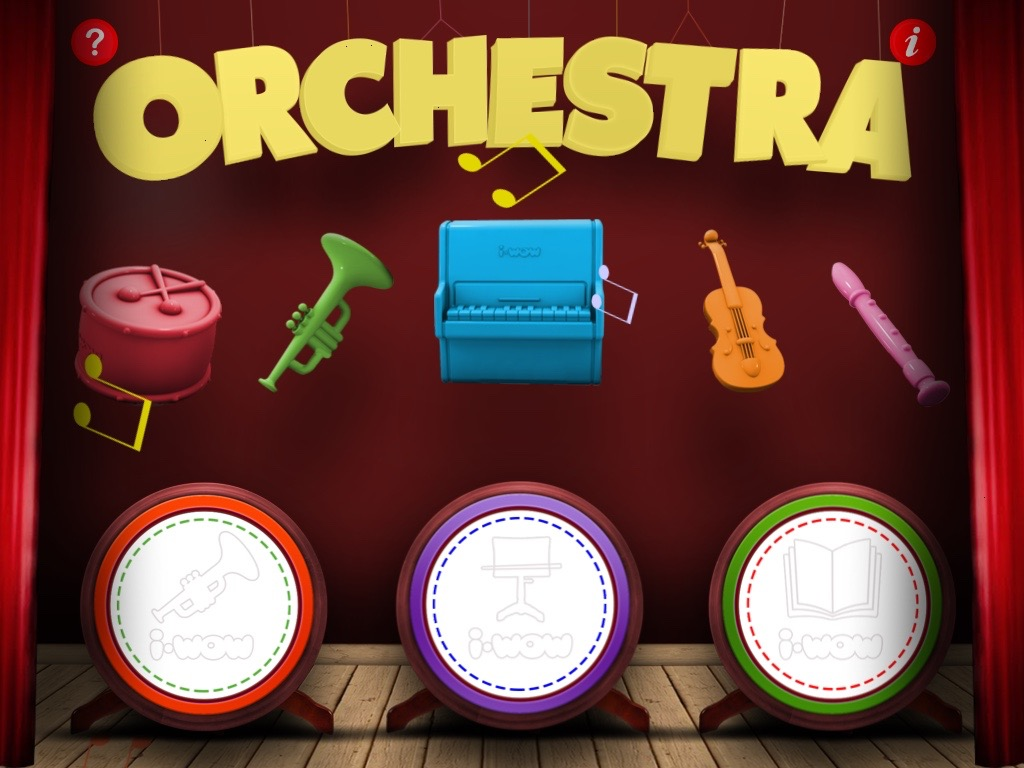
\includegraphics[width=400pt]{graphics/use-case/home_screen.jpg}
	\caption{Application Home Screen}
	\label{fig:home_screen}
\end{figure}

\newpage

By interacting with this home screen we have the possibility to access to each of the three game modes availables. In case it is our first contact with the game and we do not know how to interact with it, we can get some help touching the help button, which is represented with a question mark at the top left corner of the home screen. This help screen is shown in Figure \ref{fig:help_home_screen}.

\begin{figure}[ht!]
	\centering
	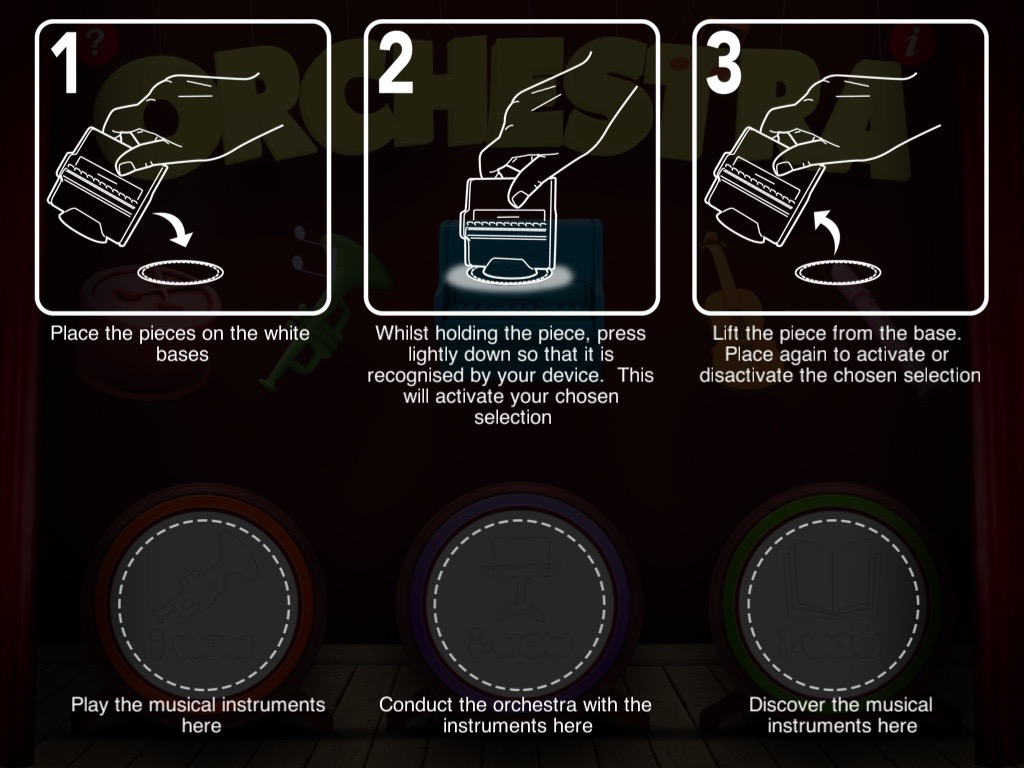
\includegraphics[width=400pt]{graphics/use-case/help_home_screen.jpg}
	\caption{Help Home Screen}
	\label{fig:help_home_screen}
\end{figure}

As we can see in Figure \ref{fig:help_home_screen}, in order to access to one of the three game modes, we should place one of the physical instrument miniature (from now on piece) on one of the instrument recognition zones (from now on white bases). After placing it, we just have to hold and press lightly down the piece so that the application can recognize it. This recognition is processed within the \textit{Instrument recognition algorithm}. After it, we can lift the piece from the white base and place another one if we want to access to another game mode after getting back to the home screen.

In this use case, we want to access to the \textit{Playing instrument game mode}, so we choose one of the pieces and place it on the left white base so that we can access to the \textit{Playing instrument game mode}. In our case, we have chosen the percussion piece. After situating the percussion piece on the left white base, a new screen, shown in Figure \ref{fig:playing_xylo_start_screen}, is opened.

\begin{figure}[ht!]
	\centering
	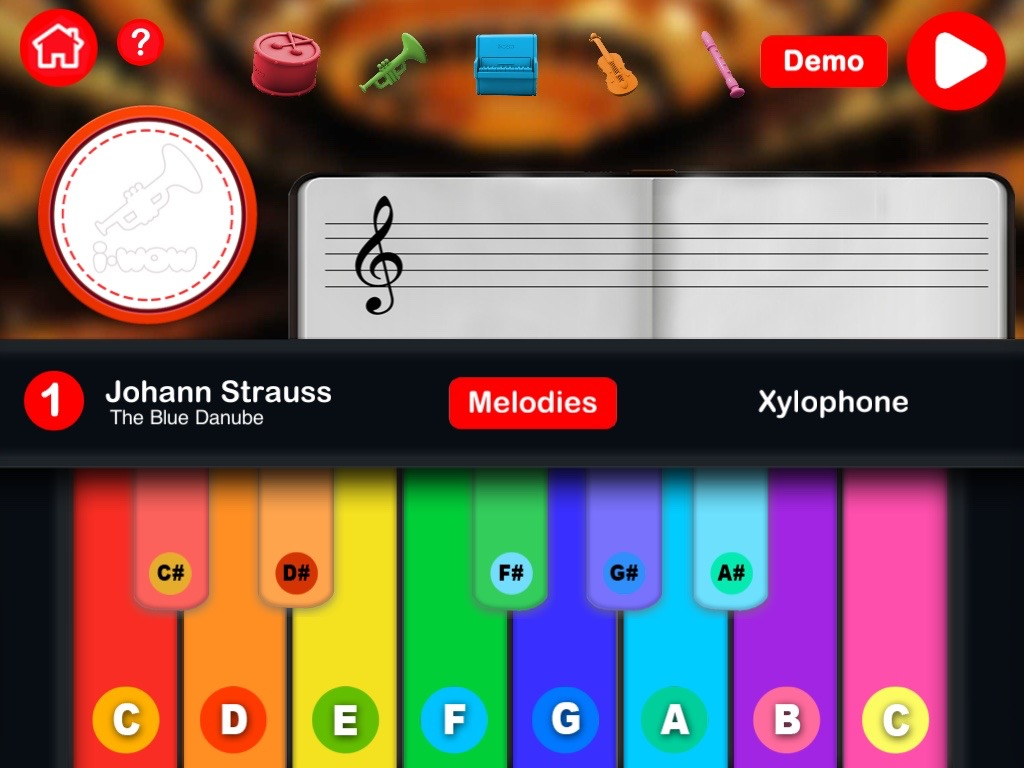
\includegraphics[width=400pt]{graphics/use-case/playing_xylo_start_screen.jpg}
	\caption{Xylophone playing instrument game mode}
	\label{fig:playing_xylo_start_screen}
\end{figure}

\FloatBarrier

In the \textit{Playing instrument game mode} screen shown in Figure \ref{fig:playing_xylo_start_screen} we can see two buttons, the \textit{Home} button and the \textit{Help} button, at the top right of the screen. These buttons allow us to get to the home application screen or to show the help information for this game mode respectively.

In Figure \ref{fig:help_playing_screen} we can take a look at the help screen information.

\begin{figure}[ht!]
	\centering
	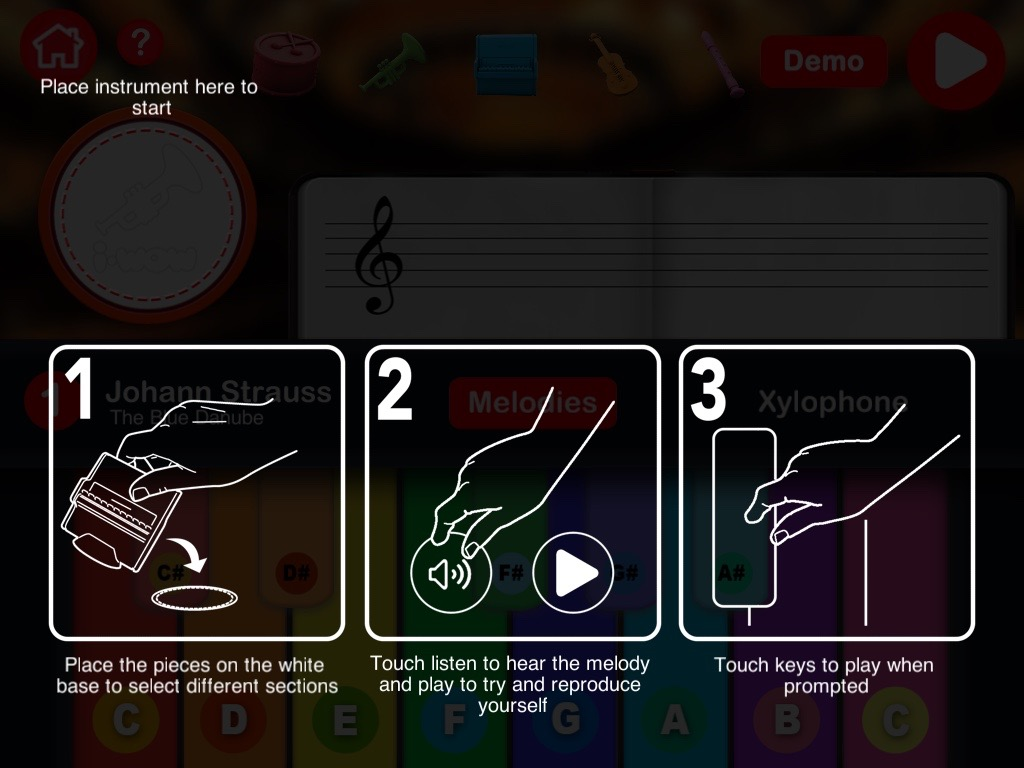
\includegraphics[width=400pt]{graphics/use-case/help_playing_screen.jpg}
	\caption{Help information playing instrument game mode}
	\label{fig:help_playing_screen}
\end{figure}

\FloatBarrier

As we can read in the help information display, we can put another instrument on the white base, located in the left of the screen, in order to select another instrument to play with. The instruments available in this game mode are the following:
\begin{itemize}
\item \textit{Xylophone}, which is selected after placing the \textit{percussion} family piece.
\item \textit{Piano}, which is selected after placing the \textit{keyboards} family piece.
\item \textit{Harp}, which is selected after placing the \textit{strings} family piece.
\item \textit{Panpipes}, which is selected after placing the \textit{woodwind} family piece.
\item \textit{Trombone}, which is selected after placing the \textit{brass} family piece.
\end{itemize}

Besides choosing an instrument we can choose the melody we are going to play. We can choose it after touching the \textit{Melodies} button placed in the center of the screen. All the melodies available in this game mode are shown in Figure \ref{fig:melodies_playing_screen}.

\begin{figure}[ht!]
	\centering
	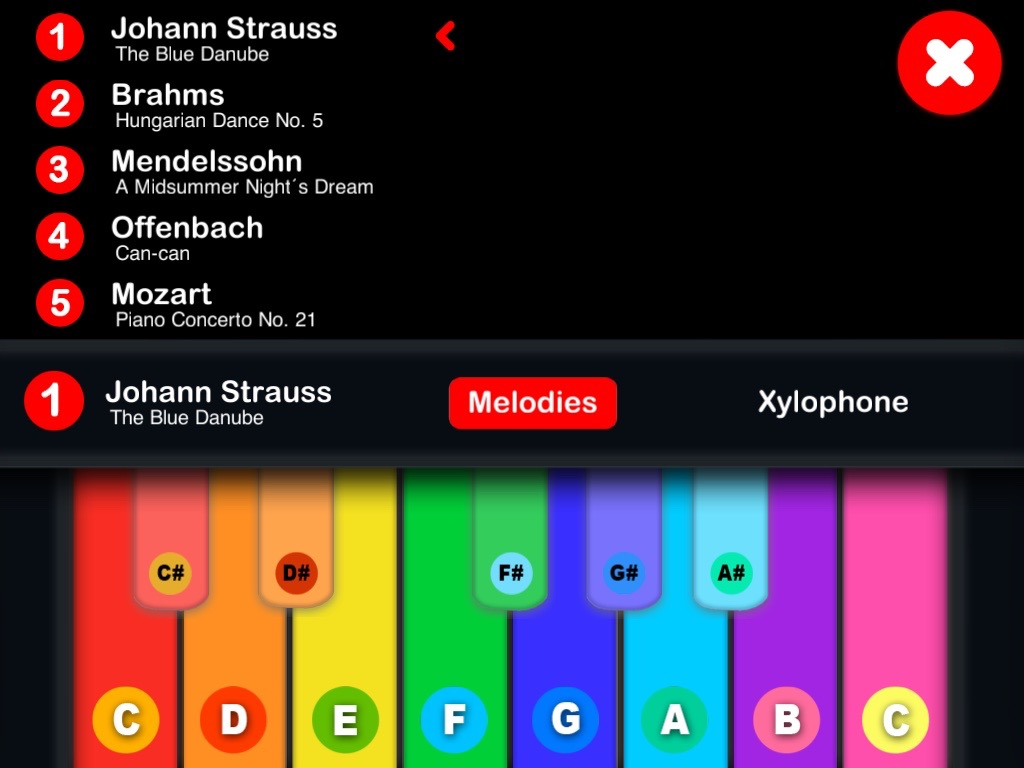
\includegraphics[width=400pt]{graphics/use-case/melodies_playing_screen.jpg}
	\caption{Melodies selection instrument game mode}
	\label{fig:melodies_playing_screen}
\end{figure}

\FloatBarrier

When we have decided which instrument we will play which melody with, we can touch the \textit{Demo} button, which is positioned in the top right of the screen. By touching the \textit{Demo} button the melody will be played automatically and the musical notes will be appearing at the sheet music placed in the center of the screen.

After watching the \textit{Demo} we are ready to play the melody with the selected instrument. We can start playing the melody by touching the \textit{Play} button located at the top right of the screen. After touching the \textit{Play} button, we have to touch the instrument keys when prompted so that we can play the whole melody. In Figure \ref{fig:play_playing_screen} we can see that the key which have to be touch is the \textit{E} key, the one that is prompted. Also, we can stop the \textit{Play mode} touching the \textit{Stop} button.

\begin{figure}[ht!]
	\centering
	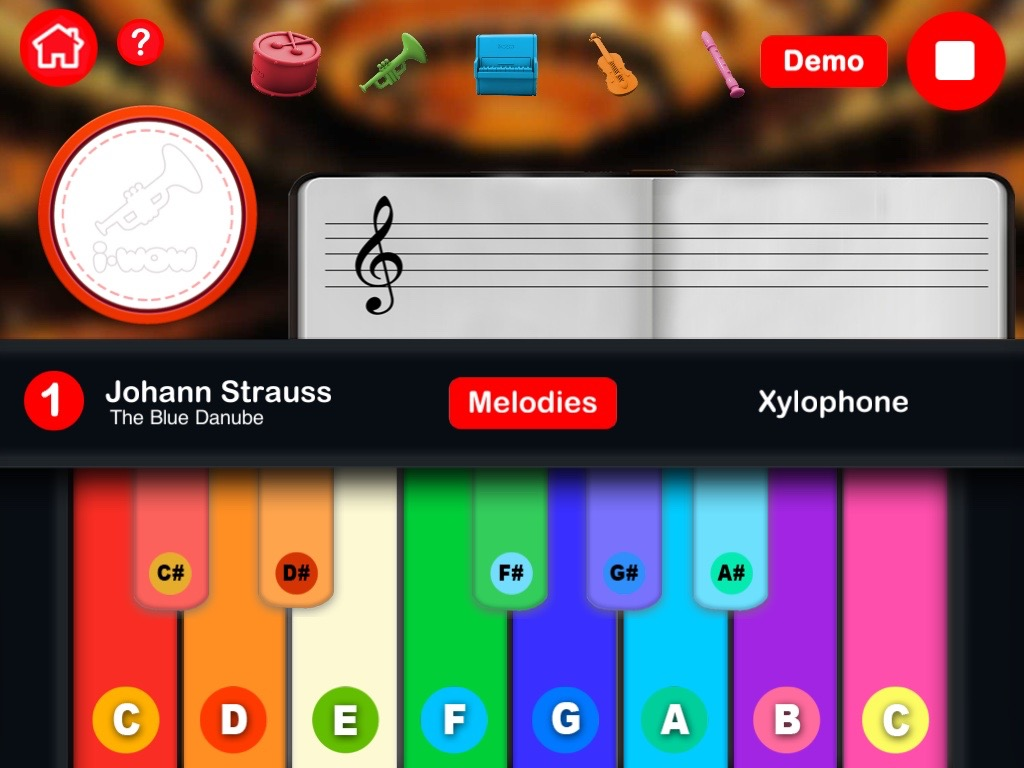
\includegraphics[width=400pt]{graphics/use-case/play_playing_screen.jpg}
	\caption{Playing instrument game mode}
	\label{fig:play_playing_screen}
\end{figure}

\FloatBarrier

Before concluding this game mode use case, we can see the rest of instrument screens in the following figures:
\begin{itemize}
\item \textit{Xylophone}, shown in Figure \ref{fig:playing_xylo_start_screen}.
\item \textit{Piano}, shown in Figure \ref{fig:playing_piano_screen}.
\item \textit{Harp}, shown in Figure \ref{fig:playing_harp_screen}.
\item \textit{Panpipes}, shown in Figure \ref{fig:playing_panpipes_screen}.
\item \textit{Trombone}, shown in Figure \ref{fig:playing_trombone_screen}.
\end{itemize}

\begin{figure}[ht!]
	\centering
	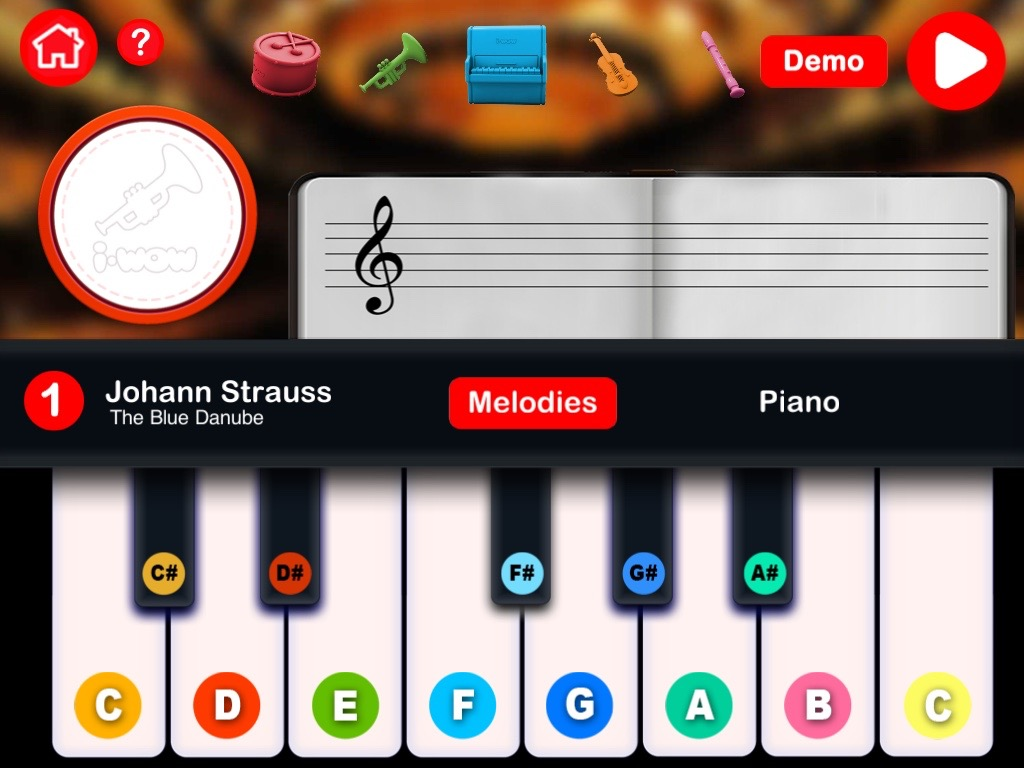
\includegraphics[width=400pt]{graphics/use-case/playing_piano_screen.jpg}
	\vspace{0.05cm}
	\caption{Playing piano screen}
	\label{fig:playing_piano_screen}

	\vspace{0.6cm}
	
	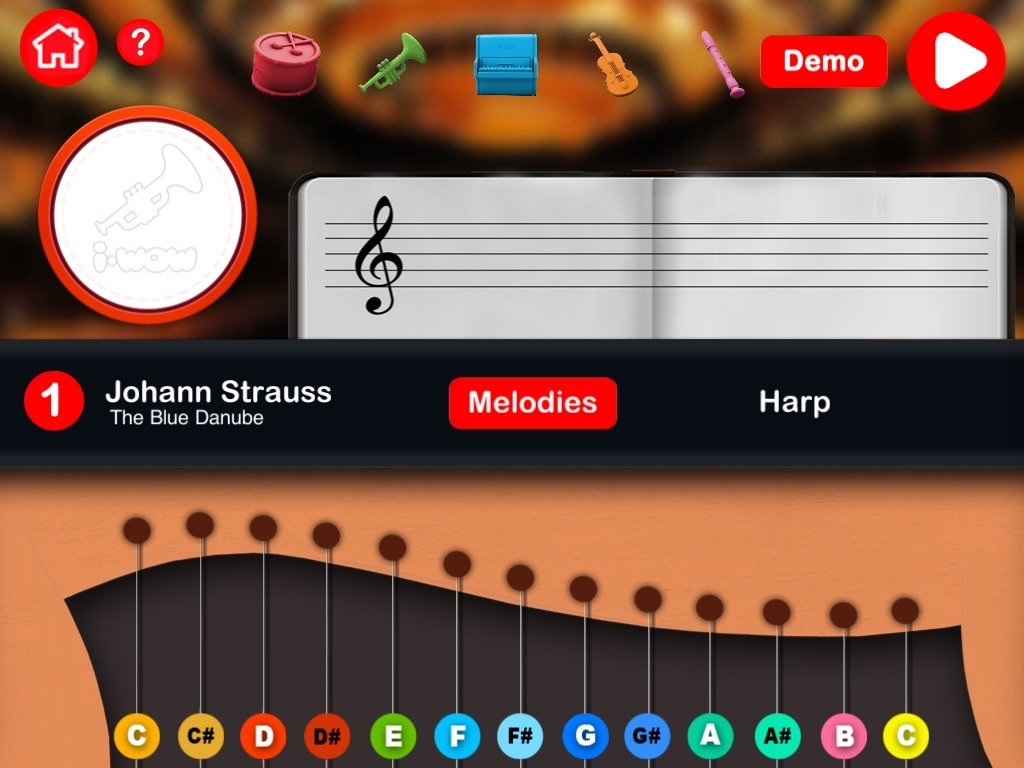
\includegraphics[width=400pt]{graphics/use-case/playing_harp_screen.jpg}
	\vspace{0.05cm}
	\caption{Playing harp screen}
	\label{fig:playing_harp_screen}
\end{figure}

\begin{figure}[ht!]
	\centering
	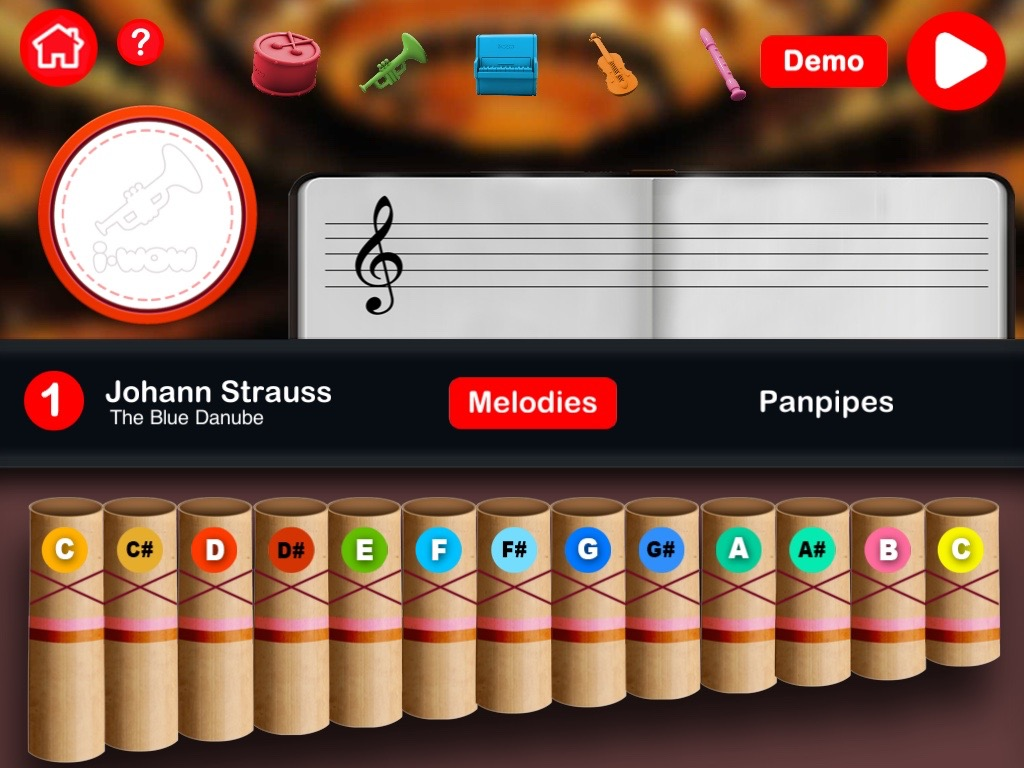
\includegraphics[width=400pt]{graphics/use-case/playing_panpipes_screen.jpg}
	\vspace{0.05cm}
	\caption{Playing panpipes screen}
	\label{fig:playing_panpipes_screen}
	\vspace{0.6cm}

	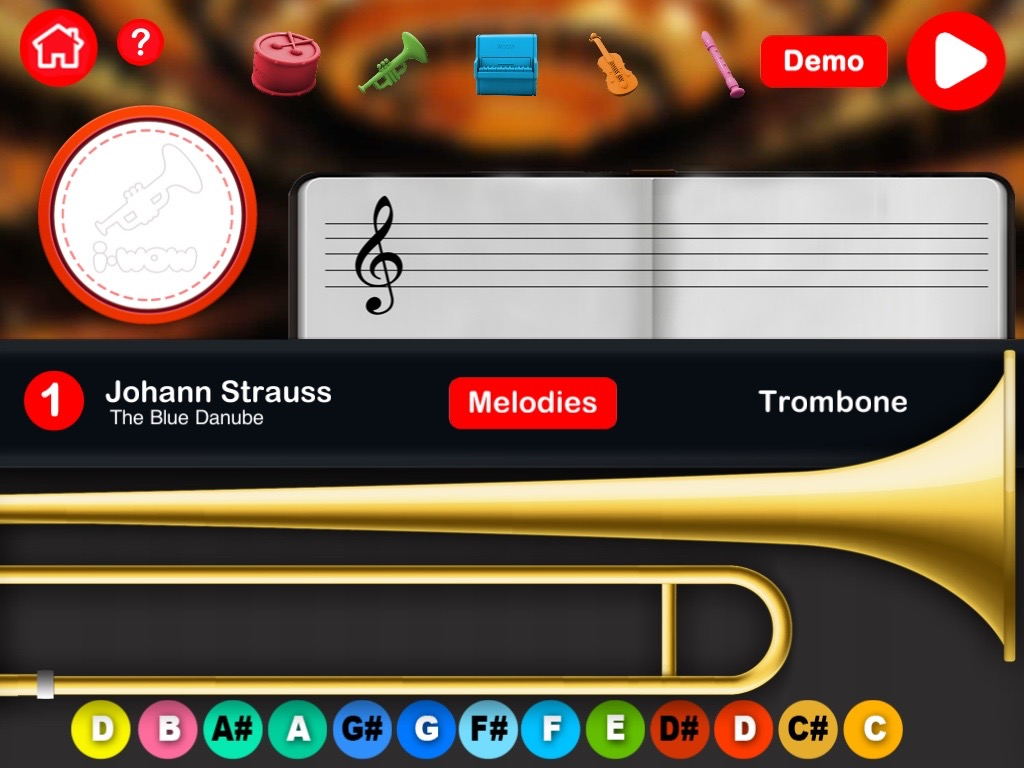
\includegraphics[width=400pt]{graphics/use-case/playing_trombone_screen.jpg}
	\vspace{0.05cm}
	\caption{Playing trombone screen}
	\label{fig:playing_trombone_screen}
\end{figure}

\FloatBarrier

\newpage
\section{Conducting orchestra game mode}
\label{sec:conductingorchestragm}

In this section we are going to detail the whole application flow within the \textit{Conducting orchestra game mode}. This game mode has been detailed in the application workflow represented in section \ref{subsec:conducteorchestra_arch}.

In order to access to this game mode, we have to proceed just as we have detailed in the previous game mode in section \ref{sec:playinginstrumentgm}.

In this use case, we want to access to the \textit{Conducting orchestra game mode}, so we choose one of the pieces and place it on the center white base so that we can access to the \textit{Conducting orchestra game mode}. After situating one of the pieces on the left white base, a new screen, shown in Figure \ref{fig:conducting_home_screen}, is opened.

\begin{figure}[ht!]
	\centering
	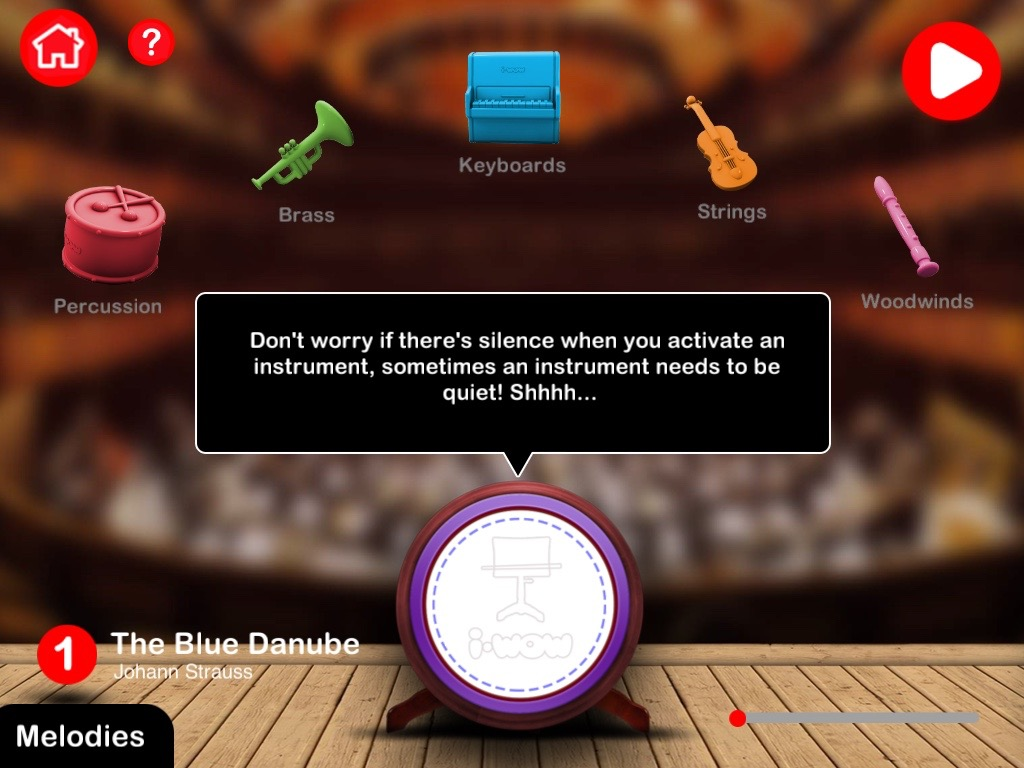
\includegraphics[width=400pt]{graphics/use-case/conducting_home_screen.jpg}
	\caption{Conducting game mode access screen}
	\label{fig:conducting_home_screen}
\end{figure}

\FloatBarrier

In the \textit{Conducting orchestra game mode} screen shown in Figure \ref{fig:conducting_home_screen} we can see two buttons, the \textit{Home} button and the \textit{Help} button, at the top right of the screen. These buttons allow us to get to the home application screen or to show the help information for this game mode respectively.

In Figure \ref{fig:help_conducting_screen} we can take a look at the help information.

\begin{figure}[ht!]
	\centering
	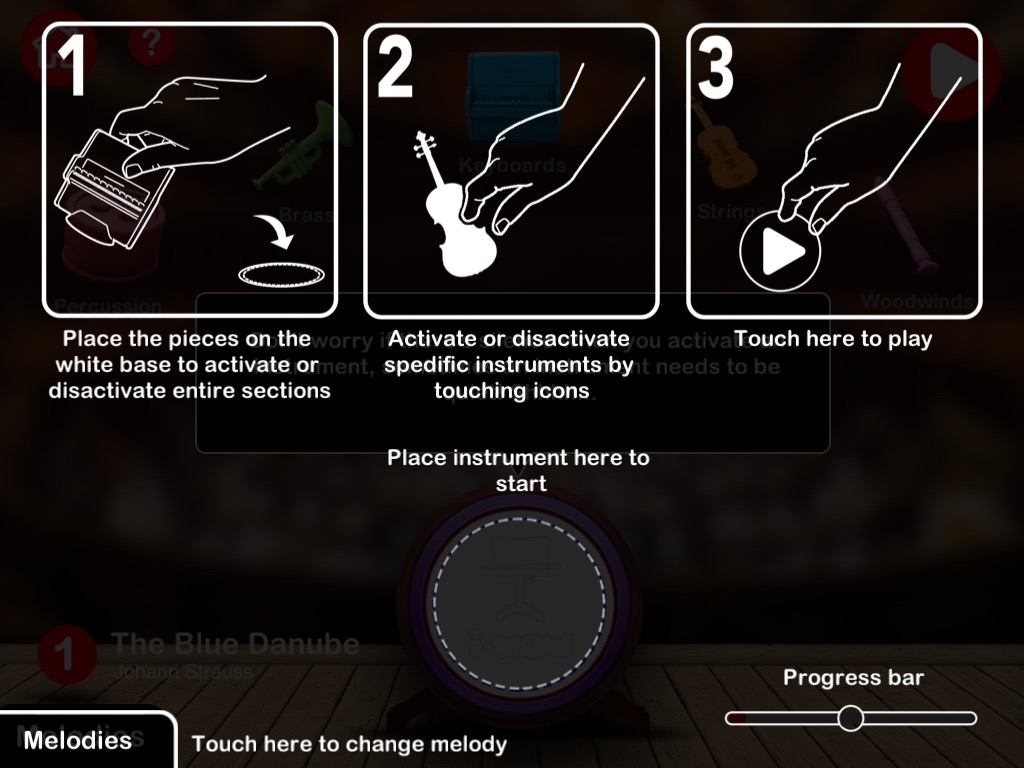
\includegraphics[width=400pt]{graphics/use-case/help_conducting_screen.jpg}
	\caption{Help information conducting orchestra game mode}
	\label{fig:help_conducting_screen}
\end{figure}

\FloatBarrier

As we can read in the help information display, we should place the instrument miniatures on the white base, located in the center of the screen, in order to activate or deactivate an instrument family section. After activating one section, we will be able to activate or deactivate the instrument belonging to the related instrument section. After choosing the what instrument we want to be activated we can touch the \textit{Play} button to start the selected melody.

When an instrument is activated, their sound will be played. So, by activating and deactivating we can conduct the musical instruments that are playing the selected melody. 

Besides conducting the orchestra, we can choose the melody played by the orchestra touching the \textit{Melodies} button placed in the bottom left of the screen. The melodies available in this game mode are shown in Figure \ref{fig:conducting_melodies_screen}.

\begin{figure}[ht!]
	\centering
	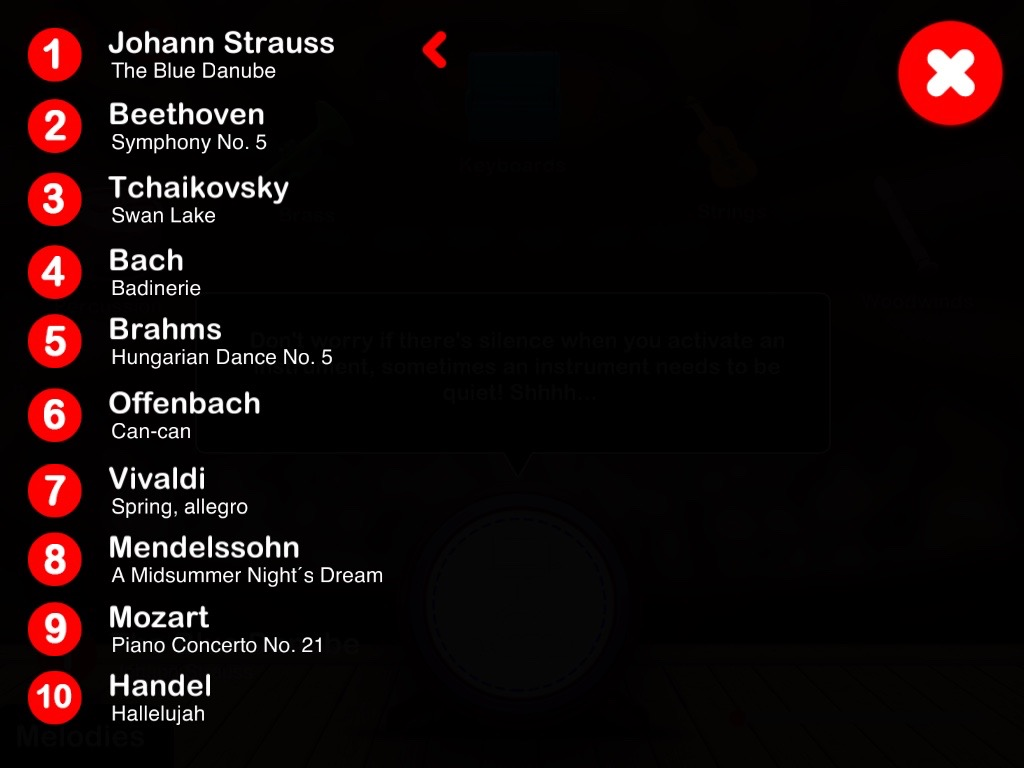
\includegraphics[width=400pt]{graphics/use-case/conducting_melodies_screen.jpg}
	\caption{Melodies selection in the conducting orchestra game mode}
	\label{fig:conducting_melodies_screen}
\end{figure}

\FloatBarrier

In Figure \ref{fig:conducting_all_stop_screen} we can see the \textit{Conducting orchestra game mode} screen where \textit{The Blue Danube} melody has been selected and all the instrument have been activated.

\begin{figure}[ht!]
	\centering
	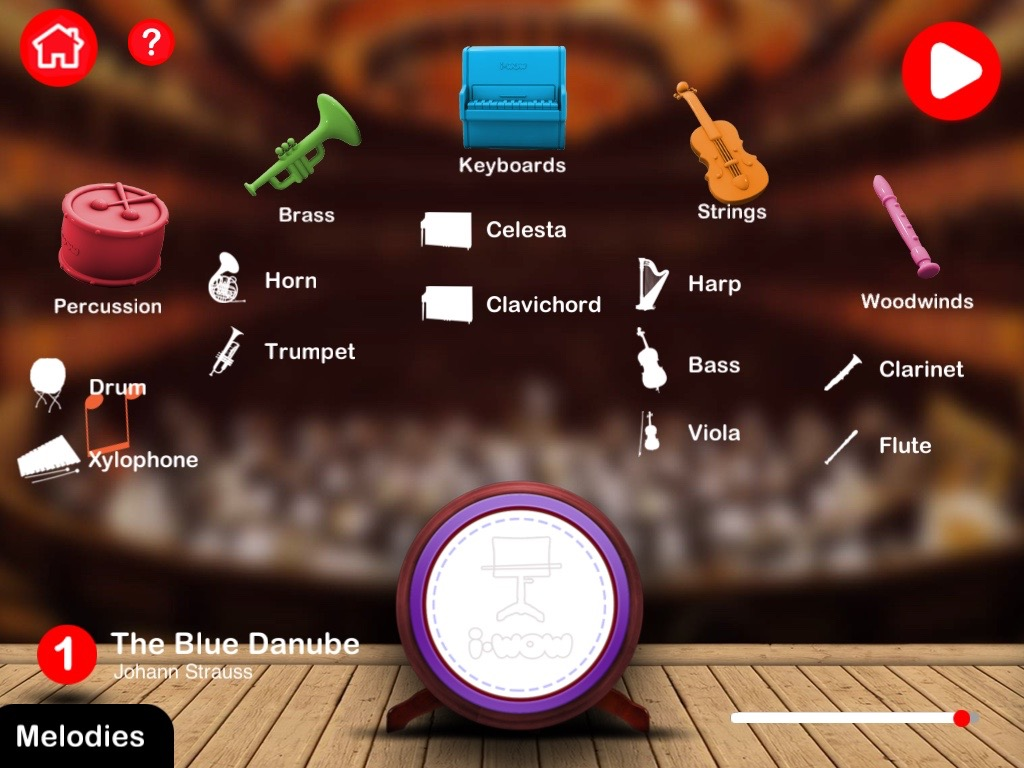
\includegraphics[width=400pt]{graphics/use-case/conducting_all_stop_screen.jpg}
	\caption{Conducting orchestra screen with all instruments activated}
	\label{fig:conducting_all_stop_screen}
\end{figure}

As we can see, there is one section for each instrument miniature that we have. The relation between the pieces and the sections is described below:
\begin{itemize}
\item \textit{Percussion section}, which is activated after placing the \textit{percussion} family piece.
\item \textit{Brass section}, which is activated after placing the \textit{brass} family piece.
\item \textit{Keyboards section}, which is activated after placing the \textit{keyboards} family piece.
\item \textit{Strings section}, which is activated after placing the \textit{strings} family piece.
\item \textit{Woodwings section}, which is activated after placing the \textit{woodwind} family piece.
\end{itemize}

\newpage

Moreover, the instruments that we can activate or deactivate within the above sections, are list below:
\begin{itemize}
\item \textit{Percussion section}: Drum and Xylophone.
\item \textit{Brass section}: Horn and Trumpet.
\item \textit{Keyboards section}: Celesta and Clavicord.
\item \textit{Strings section}: Harp, Brass and Viola.
\item \textit{Woodwings section}: Clarinet and FLute.
\end{itemize}

To end this use case, in Figure \ref{fig:conducting_some_screen} we can see the \textit{Conducting orchestra game mode} screen where \textit{The Blue Danube} melody is being played by the \textit{Xylophone}, the \textit{Celesta}, the \textit{Clavichord}, the \textit{Viola} and the \textit{Harp}, which are the instruments that have been activated.

\begin{figure}[ht!]
	\centering
	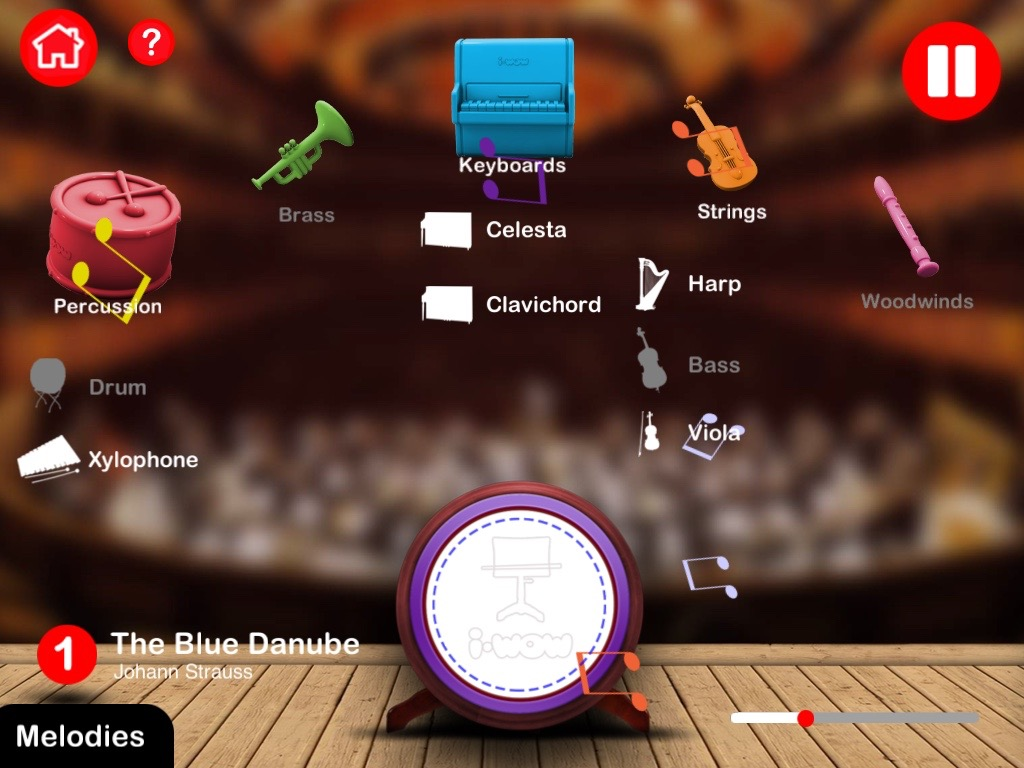
\includegraphics[width=400pt]{graphics/use-case/conducting_some_screen.jpg}
	\caption{Conducting orchestra screen with some instruments activated}
	\label{fig:conducting_some_screen}
\end{figure}

\section{Summary}
In this chapter, we detailed both \textit{Playing instrument} and \textit{Playing instrument} game modes.

Firstly, we defined the actors involved within both cases of study.

After that, we shown the game mode screen flow and hoe the gamer should interact with this game mode.
